\chapter{Advanced Tie Points}



%=======================================================================================================
\section{Tie points with low contrast images}


The current imlementation of SIFT++ used in MicMac is not fully invariant to scaling/translation in radiometry. This can create a problem with some acquisition having a good SNR but with low contrast  in the scene; in this case, due to good SNR there is potential information to get tie point, but as this information is assimilated to noise, it cannnot be exatracted.

To overcome this problem, it is possible to require that MicMac compute somme contrast enhancement on images before computing SIFT point. Also this method is not optimal (it would be better to modifiy the SIFT++ Kernel), it has the advantage of existing \dots



The figure~\ref{FIG:SF:Det} present an original image and the image after enhancement. The figure~\ref{FIG:SF:TieP} present the detected tie points; it can be seen that the spatial density is much higher. 

Of course, the enhanced images are fairly articial, as can be seen on figire ~\ref{FIG:SF:Glob} that present a full image before and after enhancement. So if this option is activated, the enhanced images are used only for the tie points steps (which are developped as specfic "hidden files" in folder {\tt Tmp-MM-Dir}).


To activate this option, the {\tt NKS-Assoc-SFS} must be changed in the {\tt MicMac-LocalChantierDescripteur.xml}. It must return {\tt SFS} instead of the default value {\tt NONE}. For example :

\begin{verbatim}
    <KeyedNamesAssociations>
        <Calcs>
            <Arrite>  1 1 </Arrite>
            <Direct>
                <PatternTransform> .* </PatternTransform>
                <CalcName>  SFS </CalcName>
            </Direct>
        </Calcs>
        <Key>   NKS-Assoc-SFS </Key>
    </KeyedNamesAssociations>
\end{verbatim}

\begin{figure}
\begin{center}
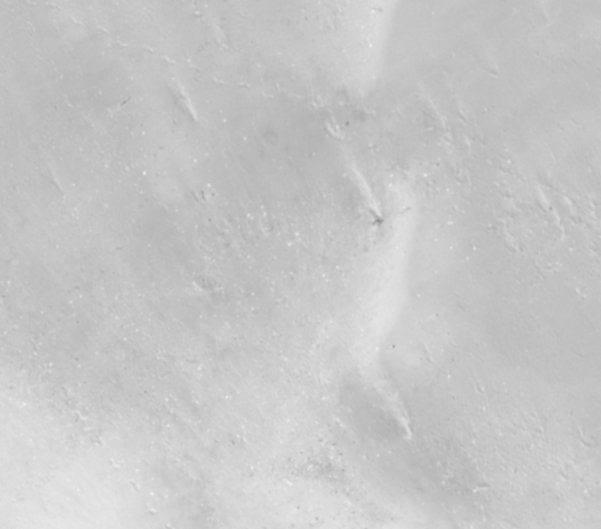
\includegraphics[width=70mm]{FIGS/Tapioca-SFS/Detail-STD.jpg}
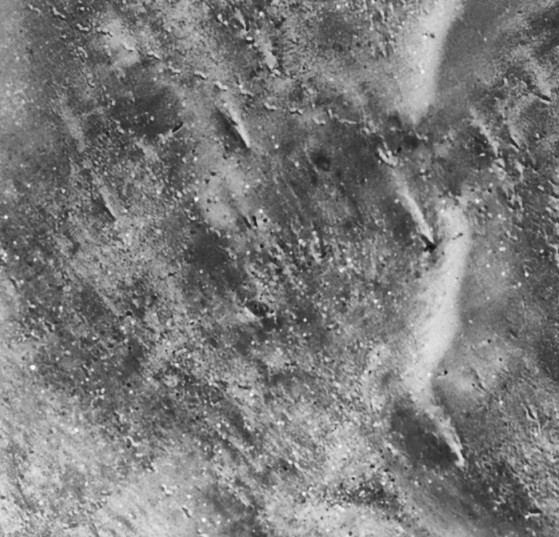
\includegraphics[width=70mm]{FIGS/Tapioca-SFS/Detail-SFS.jpg}
\end{center}
\caption{Detail of image before and after enhancement}
\label{FIG:SF:Det}
\end{figure}


\begin{figure}
\begin{center}
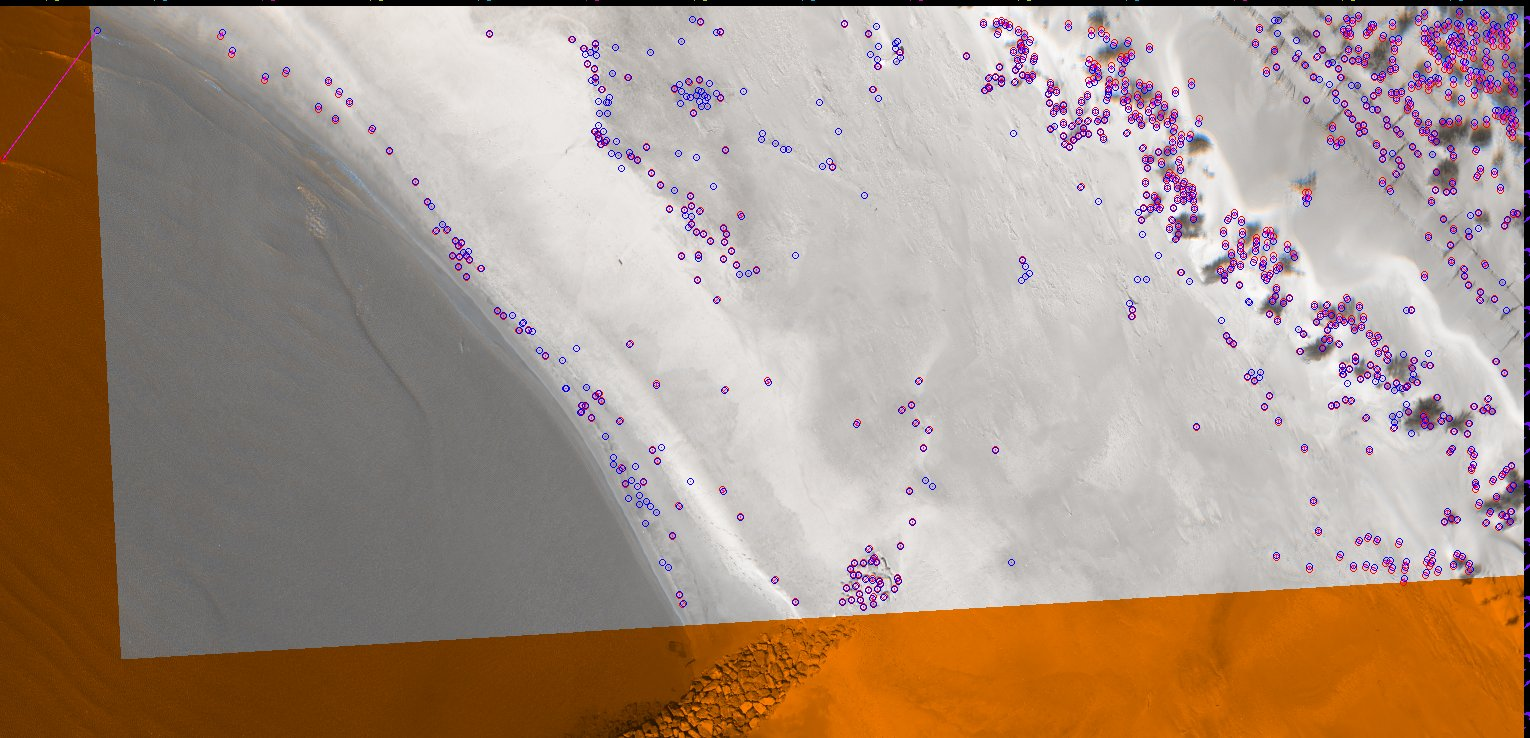
\includegraphics[width=160mm]{FIGS/Tapioca-SFS/SIFT-STD.jpg}
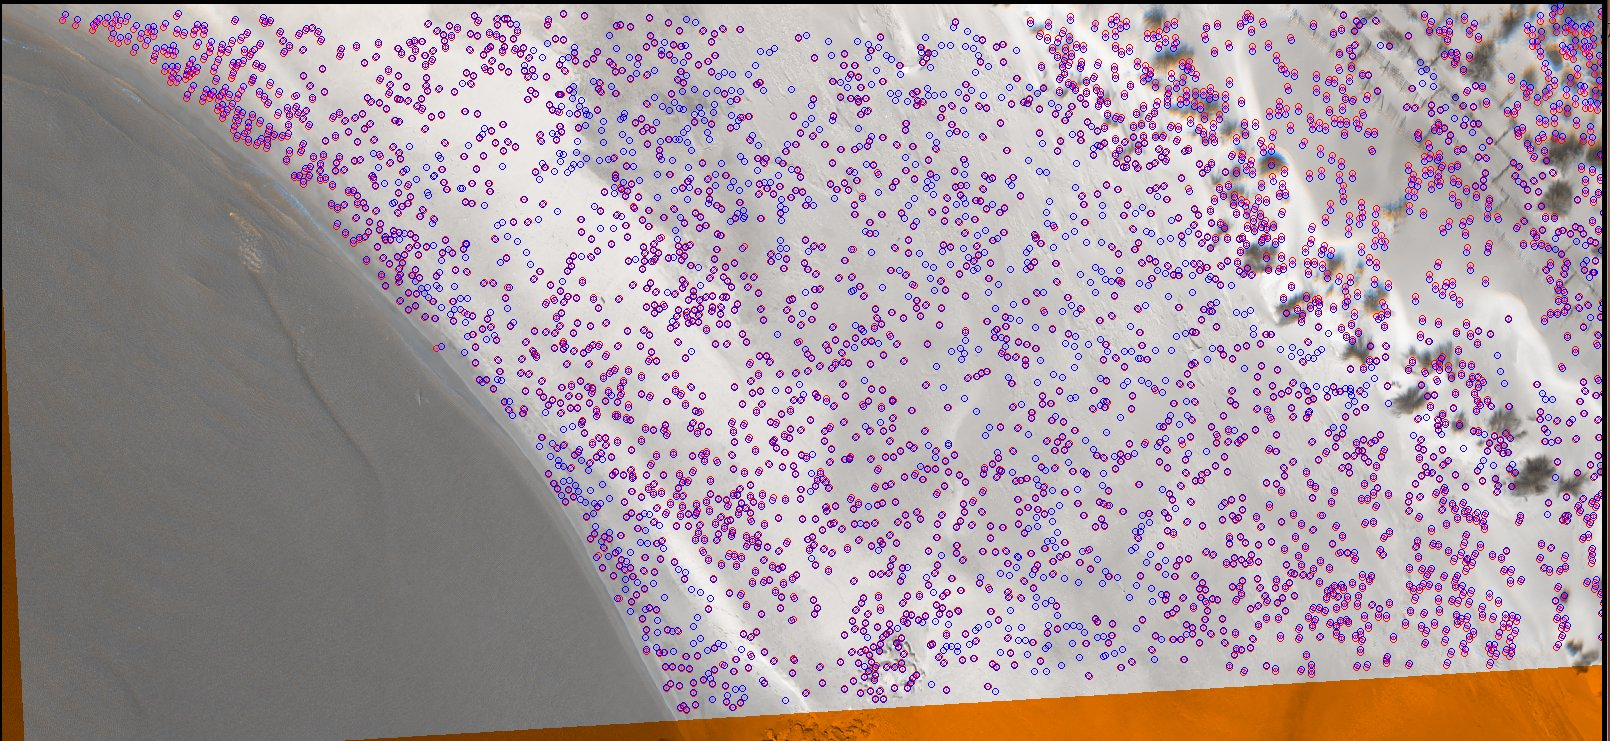
\includegraphics[width=160mm]{FIGS/Tapioca-SFS/SIFT-SFS.jpg}
\end{center}
\caption{Tie points before and after enhancement}
\label{FIG:SF:TieP}
\end{figure}

\begin{figure}
\begin{center}
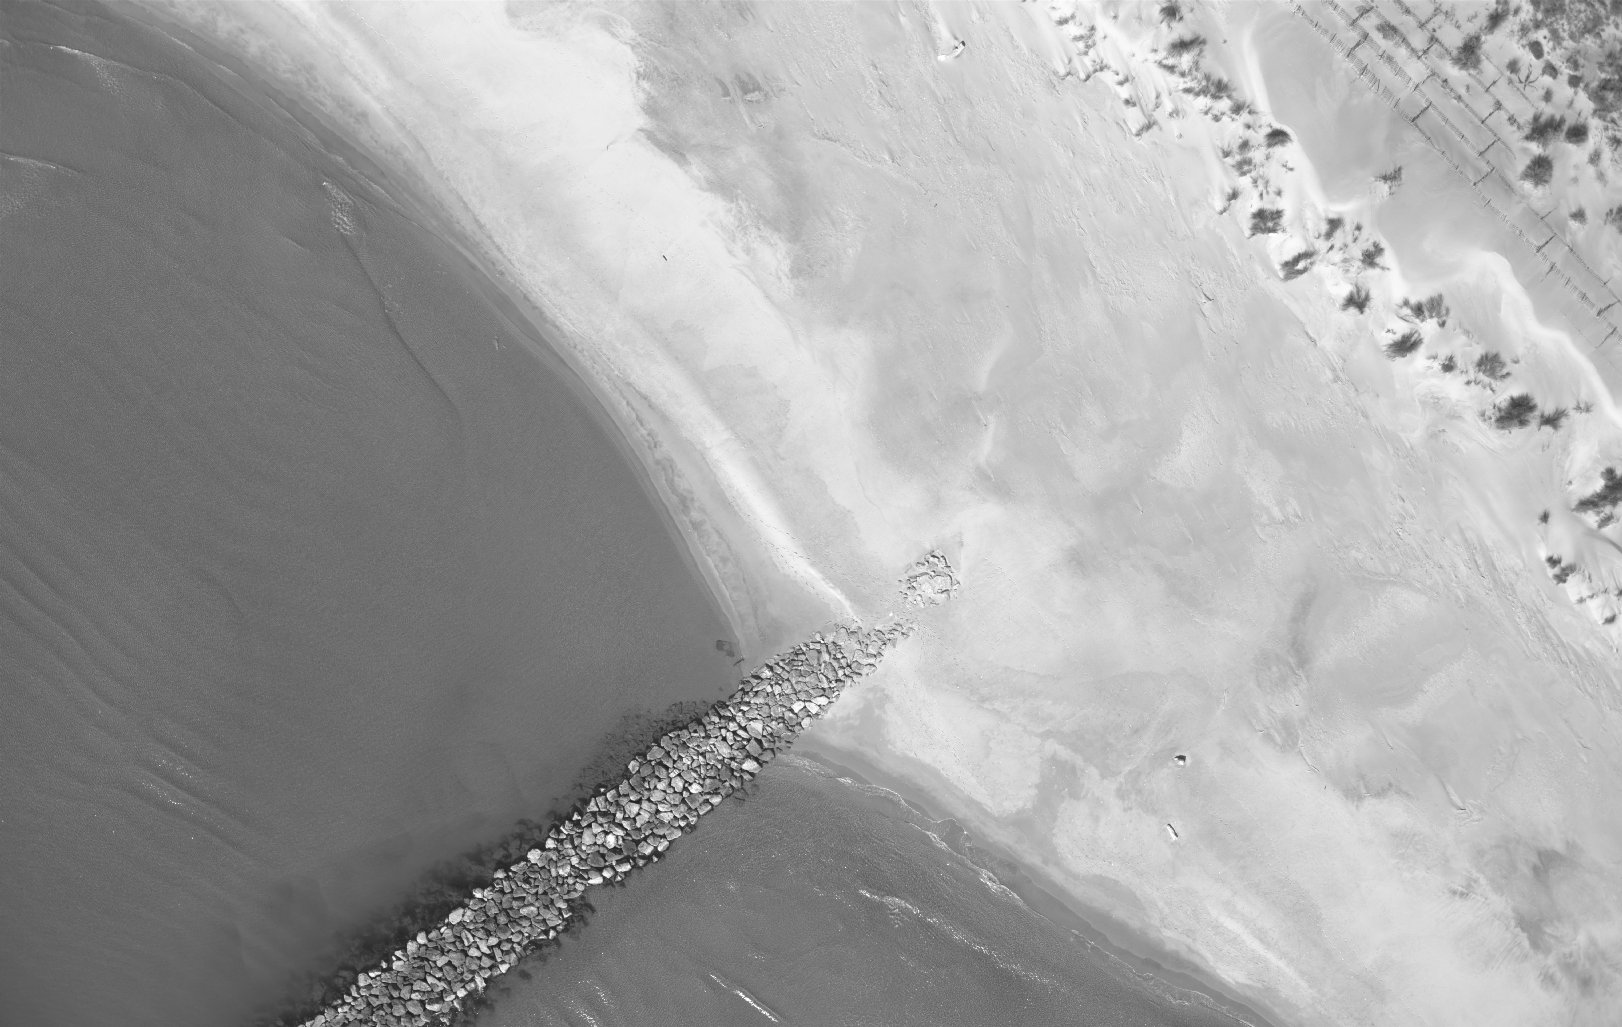
\includegraphics[width=160mm]{FIGS/Tapioca-SFS/Im-STD.jpg}
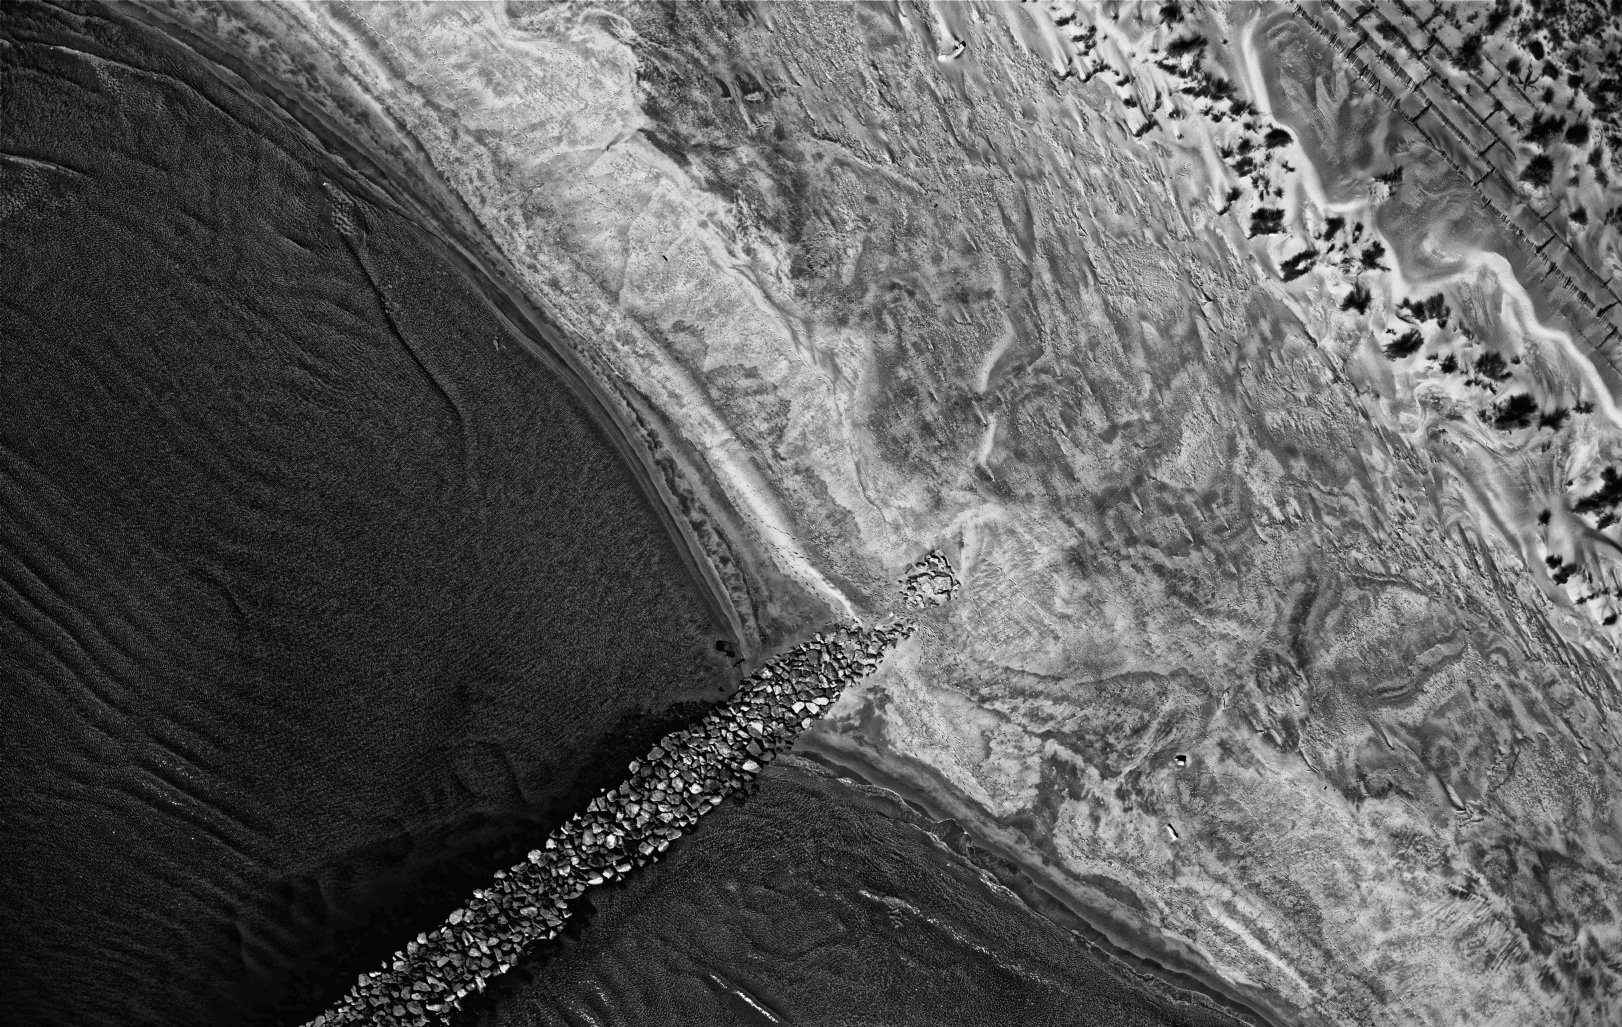
\includegraphics[width=160mm]{FIGS/Tapioca-SFS/Im-SFS.jpg}
\end{center}
\caption{Global images before and after enhancement}
\label{FIG:SF:TieP}
\end{figure}



